%%
%% static_code_analysis_in_ci.tex
%% V0.1
%% 2015/01/22
%% by 
%% Sebastian Funke
%% Hamza Zulfiqar
%% Brian Pfretzschner
%% See:
%% https://github.com/hzulfiqar/SecSoftDev
%% for current contact information.
%%


\documentclass[conference]{IEEEtran}


% *** PACKAGES ***
%\usepackage{algorithmic}
%\usepackage{array}
%\usepackage{mdwmath}
%\usepackage{mdwtab}
%\usepackage{eqparbox}
%\usepackage{fixltx2e}
%\usepackage{stfloats}
\usepackage{cite}       % http://www.ctan.org/tex-archive/macros/latex/contrib/supported/cite/
\ifx\pdfoutput\undefined
\usepackage{graphicx}   % http://www.ctan.org/tex-archive/macros/latex/required/graphics/
\else
\usepackage[pdftex]{graphicx}
\fi
\usepackage{subfigure}  % http://www.ctan.org/tex-archive/macros/latex/contrib/supported/subfigure/
\usepackage{url}        % http://www.ctan.org/tex-archive/macros/latex/contrib/other/misc/
\usepackage[cmex10]{amsmath}    % http://www.ctan.org/tex-archive/macros/latex/required/amslatex/math/
%\usepackage{amsfonts}
\interdisplaylinepenalty=2500
\ifx\pdfoutput\undefined
\usepackage[hypertex]{hyperref}
\else                   % http://www.ctan.org/tex-archive/macros/latex/contrib/supported/hyperref/
\usepackage[pdftex,hypertexnames=false]{hyperref}
\fi
\usepackage[colorinlistoftodos,prependcaption,textsize=tiny]{todonotes}
\usepackage{listings}
\lstset{frame=single}

% correct bad hyphenation here
\hyphenation{op-tical net-works semi-conduc-tor}

\begin{document}
%
% paper title
\title{Integration of Static Security Code Analysis\\in Continuous Integration Lifecycles}



%\author{\IEEEauthorblockN{Sebastian Funke}
%\IEEEauthorblockA{Secure Software Engineering\\
%TU Darmstadt\\
%sebastian.funke@stud.tu-darmstadt.de}
%\and
%\IEEEauthorblockN{Brian Pfretzschner}
%\IEEEauthorblockA{Secure Software Engineering\\
%TU Darmstadt\\
%brian.pfretzschner@stud.tu-darmstadt.de}
%\and
%\IEEEauthorblockN{Hamza Zulfiqar}
%\IEEEauthorblockA{Secure Software Engineering\\
%TU Darmstadt\\
%hamza.zulfiqar@stud.tu-darmstadt.de}}



\author{\authorblockA{Sebastian Funke, Brian Pfretzschner, Hamza Zulfiqar}
	\authorblockA{Center for Advanced Security Research Darmstadt\\
		Department of Computer Science\\
		Technische Universit\"at Darmstadt, Germany}}




% use for special paper notices
%\IEEEspecialpapernotice{(Invited Paper)}




% make the title area
\maketitle


\begin{abstract}
\boldmath
Static code analysis should run frequently in an continuous integration lifecycle. Each run produces lots of information that need to be reviewed, evaluated and integrated in the ongoing development process. Therefore, the analysis results should be reworked, concentrated and presented in a helpful manner.
\end{abstract}

% no keywords

% For peerreview papers, this IEEEtran command inserts a page break and
% creates the second title. It will be ignored for other modes.
\IEEEpeerreviewmaketitle



\section{Introduction}
% no \IEEEPARstart
\todo[inline]{Content from our slides...about input validation and how static code analysis works.
Limitation on open source, static analysis tools. Jenkins, SonarQube...and why.
Content of our paper, what comes when blabla...}
\cite{SecurityinCI}

Building secure software systems gets more and more important. Not just private hackers are attacking our software, also foreign and even western governments put in great effort in breaking into important systems\cite{NSAHacking}.


Therefore we have to improve the software development process in terms of early and continuous security analysis of the source code.
Such static analysis tools can be applied independently during the development process at different stages.
One option would be the integration of analyzers within the IDE of the developer.
Another possibility is the combination of those tools in a continuous integration system, to collect issues during or after the build process.
Besides CI, IDE and the development tool chain can be extended with code quality management systems, as platform for analyze the code and manage the analyzed issues.


In our paper, we compare and evaluate the issue reporting capabilities in two CI tools (Jenkins and Teamcity), two code quality management tools (SonarQube, Codeclimate) and the IDE Eclipse.
We integrated the popular analyzers FindBugs and PMD in each development tool above and executed them on a Java test project (JEdit\footnotetext{http://www.jedit.org/}) with a variety of issues.


We address that what needs validation, how to perform input validation and how to respond when an input fails an authentication check. Furthermore, we analysed how input validation is deployed in popular PHP frameworks.





\todo[inline]{Outline with section numbers (explain the structure of the paper)}


\subsection{Types of Analyzers}
There are different types of analyzers which all have a different scope. Most of them are specialized to a specific programming language, but some are also capable of analyzing multiple languages. An example for a multi-language analyzer is \href{http://pmd.sourceforge.net/pmd-4.3.0/cpd.html}{CPD} (Copy/Paste Detector) which is supposed to find duplicate code. It works with Java, JSP, C, C++, Fortran and PHP code.


Furthermore it is important to distinguish when to apply analyzers in the Software Development Lifecycle.
Most analyzer exist as stand-alone version and allow the integration in common development tools, like IDE's and CI tools.


Advantages of Continuous Integration (CI)\cite{SecurityinCI}:
\begin{itemize}
	\item \textit{Immediate Notification}
	CI ensures that ongoing changes to the source code do not break the intent or design of the software. If a change does break the software, that break is identified immediately and can be fixed with a minimal cost and impact to the projects schedule.
	
	\item \textit{Secure Development}
	By integrating security testing and secure code analysis, CI can be further leveraged to include secure development practices while minimizing the amount of extra effort required to get the benefits of secure development. Since it is tied to CI,
	security testing and secure code review begins when a project begins and runs continuously
	throughout project development. With CI, security vulnerabilities testing becomes part of the regression test bed, executed automatically with each successive build on the CI platform.
	
	\item \textit{Trend and History}
	CI enables a higher management layer to view the history and trend of issues and builds.
	
\end{itemize}


\subsection{Candidates to manage Static Code Analysis}
\label{subsec:candidates-to-manage-static-code-analysis}
We decided for the following tools, as possible candidates to manage static code analysis on software projects.


\subsubsection{Eclipse}
\label{subsubsec:eclipse}


\subsubsection{Jenkins}
\label{subsubsec:jenkins}
Jenkins is a widely used tool to control and manage continuous integration tasks. Its main purpose is to monitor the execution of repeated jobs and present their outcomes.\footnote{From Jenkins Website, \href{https://wiki.jenkins-ci.org/display/JENKINS/Meet+Jenkins}{Meet Jenkins}}

\subsubsection{Teamcity}
\label{subsubsec:teamcity}



\subsubsection{SonarQube}
\label{subsubsec:sonarqube}
SonarQube is an OpenSource project, implemented as web application within its own webserver, with the aim to analyze and manage the quality of source code. 
Besides analysis against common coding guidelines, like duplicate code, missing comments and potential bugs, it also checks for several security issues (e.g. from the OWSASP Top 10 list).
Therefore it provides a central place to manage intuitively analysis rules from different analyzer extensions.
The main difference to CI tools, is the feature to manage the found issues.
Over plugins it is possible to extend the analysis scope to over 20 programming languages.


\subsubsection{Codeclimate}
\label{subsubsec:codeclimate}



\section{Input validation in popular frameworks}
\label{sec:input_validation}
\todo{Move this section to the end? - Brian}
Check those \url{http://codegeekz.com/20-best-php-frameworks-developers-august-2014/} and make a table how input validation is handled there...
The most common security weakness in any application is the failure to properly validate input from the environment. This weakness further leads to almost all of the major vulnerabilities in applications, including buffer overflow, SQL injection and a whole lot more. So, the maximum essential cautious measure that developers can take is to comprehensively authenticate the input that a software obtains. Certainly programs need to accept input, and computing a decent result depends on having a good input. There is a misconception that input can be trusted just because it is coming from some so-called trusted source. Input must not enter into the system without passing through various security methods.



\section{Static code analysis in IDE}
\label{sec:static_code_analysis_ide}

\todo[inline]{Write about findbugs and pmd integration in eclipse, how, pro and con...}



\section{Static code analysis in CI}
\label{sec:static_code_analysis_ci}

\subsection{Jenkins}
\label{subsec:jenkins}
Used test suite: wireshark 1.8 from NIST testsuites with 85 vulnerabilities.
Because its C, because its one of the most security critical languages and there are many good analyzers for C.
Why not Juliet TestSuite with 65 000 vulnerabilities?
Because they are collections of testcases and not a easily build-able project and the analysis and build process would take to long to evaluate the reporting features of the analyzers.

\todo[inline]{Table with Jenkins Analyzer Plugins (below) with pros and cons}


\begin{figure}[!t]
	\centering
	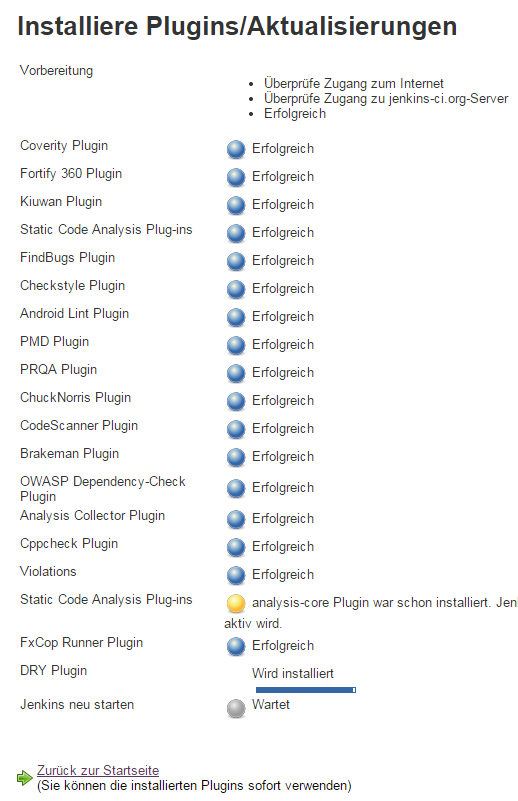
\includegraphics[width=1\linewidth]{img/jenkins-code-analysis-plugins.png}
	\caption{Just a few used Jenkins plugins for static code analysis}
	\label{fig:jenkins-plugins}
\end{figure}


\subsection{Teamcity}
\label{subsec:static_code_analysis_teamcity}
\begin{itemize}
	\item Installation: The Teamcity installation was a bit easier than Sonarqube because the database connection was configured in a wizard and similar it consists out of a webserver with webinterface (localhost:8111) and a database.
	
	\item Language support: All (since it is a highly customizable CI tool)
	
	\item Rule Management: The analyzers have to run externally and Teamcity will import the analysis results.
	Hence, it is much effort to configure and install different analyzers with different rulesets.
	
	\item Issue-Presentation: In the build details you can show issues in the Code Inspection tab, what present just the xml tree of the parsed reports, no filter options, no resolve options, no severity levels.
	
	\item Positive: Better user interface than Jenkins. With installed IDE plugin, you can jump to issue source-code directly in the IDE. 
	
	\item Negative: Hard to configure the external pmd and findbugs reports. Visualization of issues very limited. Two different inspections can not be processed during one build (skipped PMD report)
	
\end{itemize}





\section{Static code analysis in code quality management}
\label{sec:static_code_analysis_code_quality_management}

\subsection{SonarQube}
\label{subsec:sonarqube}
\begin{itemize}
\item Installation: Sonarqube consists out of 3 parts: the local webserver (localhost:9000), a database to load and store analysis results and the sonarqube runner, which analyses the code specified in a project property file.

\item Language support: Java and other languages available as plugins

\item Rule Management: Very intuitive and easy to configure rules for so called quality profiles. Very interesting, that you can manage the rules of all analyzer plugins in one menu. It comes already with default sonarqube rules with different severity levels, detailed descriptions in different categories. Also including security relevant rules e.g. from OWASPTop10 and CWEs. One can compose a static analysis out of those rules including rules from plugins like FindBugs and PMD.

\item Issue-Presentation: Dashboard as starting point presents overview very well with different informative metrics, mostly for code quality and presents the number of issues of the different severity levels.
In the menu issues and issue-drilldown one can sort the issue list, search for issues matching to specific rules and get more information to the issue and most important where the issue is located in the code.

\item Positive: Good overview over issues, fast analysis, good rule management, good issue management with assigning issues to users etc.

\item Negative: In Rule-Management one can filter rules by tags and categories (bugs, security bugs), but you can not use those filters in the issue management. This leads to a big list of issues where you cant distinguish e.g. between a unused code and security issue.
 
\end{itemize}

We subdivide our evaluations by programming language because the analyzers and their main purpose differs heavily in respect to their target language.

\section{C/C++}

\subsection{Cppcheck}
\textit{Cppcheck} is a very powerful analyzer for C and C++ which can find a lot different code issues. For example it tries to find out-of-bounds accesses, memory leaks or warn if obsolete or unsafe functions are used. Its main goal is to avoid false positives.

Cppcheck is easy to use and can be integrated in an continuous life cycle with very little effort.
Listing \ref{lst:cppcheck} shows how to run a Cppcheck analysis on C/C++ project. When you use this command, Cppcheck will run with 4 threads (\texttt{-j 4}), does all analysis it supports (\texttt{--enable=all}) and writes the results as xml file on disk after it examined any C/C++ file in the current folder and any folder below that (recursively).

\begin{lstlisting}[caption={Bash command to run Cppcheck},label={lst:cppcheck}]
$ cppcheck -j 4 --enable=all \
	--xml --xml-version=2 . \
	2> cppcheck.xml
\end{lstlisting}


\subsubsection{Cppcheck \& Jenkins}
There exists a dedicated \href{https://wiki.jenkins-ci.org/display/JENKINS/Cppcheck+Plugin}{Jenkins plugin for Cppcheck}. This plugin does not include the Cppcheck analysis. This has to be performed as a build step which produces a XML-file containing the analysis results. The plugin will then, as a post-build task, read the XML-file and display the contents in a processed manner.

\subsubsection{Cppcheck \& SonarQube}


\subsection{Codeclimate}
\label{subsec:codeclimate}



\section{Evaluation of reporting capabilities}
\label{sec:evaluation}
We decided to make a qualitative evaluation, with usability inspection heuristics described in the book Information Visualization by Kerren et al. \cite{InformationVisualizationBook}.
From the work of Hollingsed et al. on 15 years of usability inspection evaluation \cite{15yearsUsabilityEvaluation}, we derived the best method would be a combination of a cognitive walk-through, combined with the usability heuristic evaluation defined by Nielsen \cite{Nielsen:UsabilityInspectionMethods}.
This wide-used, informal, very cost efficient and effective method is proven to find with a appropriate skilled evaluator team 55 - 90\% of all usability problems.


The usability inspection over heuristic evaluation method uses a small group of usability experts, who evaluate a
user interface using a set of guidelines and noting the severity of
each usability problem and where it exists. 
We combine it with a cognitive walk-though, in the way, that three experts go through the tools with a cognitive expected path in context of applying static code analysis with an additional usability guidelines list for every stage.


We identified four stages of our walk-through and evaluate several usability guidelines in each stage:

\begin{itemize}
	\item Prepare analysis
	\begin{itemize}
		\item Is the tool easy and intuitive to configure?
		\item Is it possible to add external analyzers?
		\item Is it possible to configure the analyzers?
	\end{itemize}
	\item Run analysis
	\begin{itemize}
		\item ...
	\end{itemize}
	\item Evaluate analysis results
	\item Manage analysis results
\end{itemize}


\subsection{Eclipse}
\label{subsec:evaluation_eclipse}

\subsection{Jenkins}
\label{subsec:evaluation_jenkins}

\subsection{Teamcity}
\label{subsec:evaluation_teamcity}

\subsection{SonarQube}
\label{subsec:evaluation_sonarqube}

\subsection{Codeclimate}
\label{subsec:evaluation_codeclimate}


\subsection{Comparation}
\label{subsec:comparation}



\section{Conclusion}
\label{sec:conclusion}
\begin{itemize}
	\item Conclusion about how input validation is done in frameworks, what can be better ...
	\item Conclusion, is it better to integrate static analysis in Jenkins or just use SonarQube
	....its really not that easy to find the right static code analyzer for your project with a specific programming language. There are lots of open source tools, but very old and just supported by Jenkins over hacks.
	\item Conclusion, is reporting in Jenkins useable? No...just in combination with code quality management tools
	\item Future work: Using many tools is basically a good idea, because more tools find potentially more vulnerabilities. A future approach would be to implement a tool that can filter all the generated reports. Thereby duplicate vulnerabilities findings can be merged and false positives can be reduced.
\end{itemize}






\section{Sources and useful links}
\begin{itemize}
	\item \href{http://www.crosstalkonline.org/storage/issue-archives/2010/201003/201003-Stiehm.pdf}{Building Security In Using Continuous Integration}
	\item \href{http://www.jetbrains.com/teamcity}{TeamCity}\\
	Supports static code analysis. Also, it can import analysis reports produced by these tools: PMD, PMD/CPD, FindBugs, Checkstyle or JSLint.
	\item \href{http://jenkins-ci.org}{Jenkins}
	\item \href{http://continuum.apache.org}{Apache Continuum}	
	\item \href{http://codeclimate.com}{codeclimate.com}
\end{itemize}

\bibliographystyle{IEEEtran}
% argument is your BibTeX string definitions and bibliography database(s)
\bibliography{references}

\end{document}


